\begin{frame}{Teorema Principal}
    \begin{thm}[\cite{Cygan15, Will11}]
        \label{teo:2}
        Existe um algoritmo que, dada uma instância $I=(G, k)$ do problema CI em que $G$ é planar, resolve $I$ em tempo $2^{O(k)} \cdot n^{O(1)}$.
    \end{thm}
\end{frame}

\begin{frame}{Observação}
    \centering
    \vspace{1cm}
    \pause
    \Large Assim como ogros, grafos planares têm camadas!
    \begin{minipage}{\linewidth}
        \centering
        \vspace{1.73cm}
        
\includegraphics[height=5cm]{images/shrek.png}
    \end{minipage}
\end{frame}

\begin{frame}{Relembrando}
    \begin{minipage}{\linewidth}
        \centering
        \only<1>{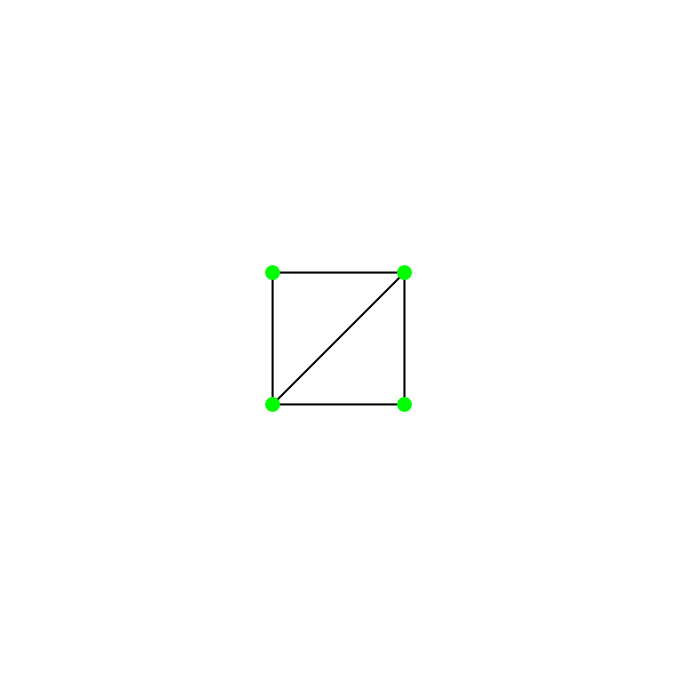
\includegraphics[height=6cm]{images/outer1.png}}
        \only<2>{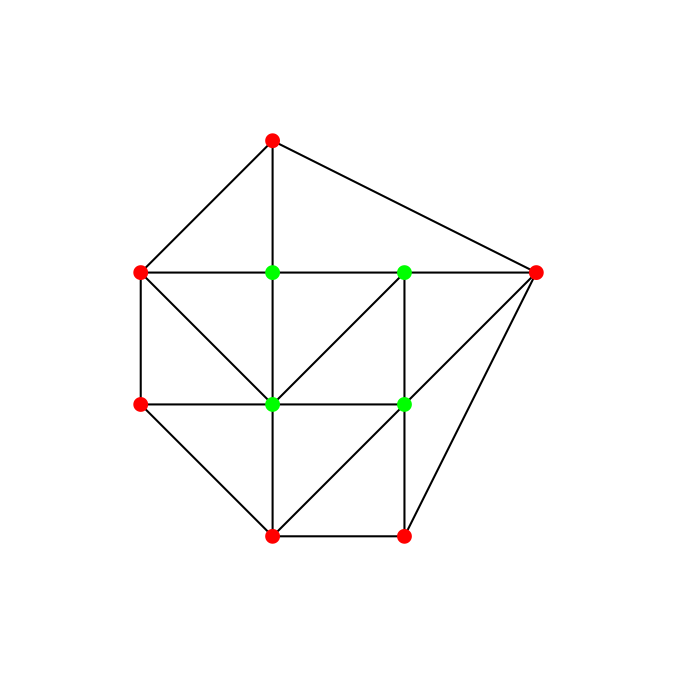
\includegraphics[height=6cm]{images/outer2.png}}
        \only<3>{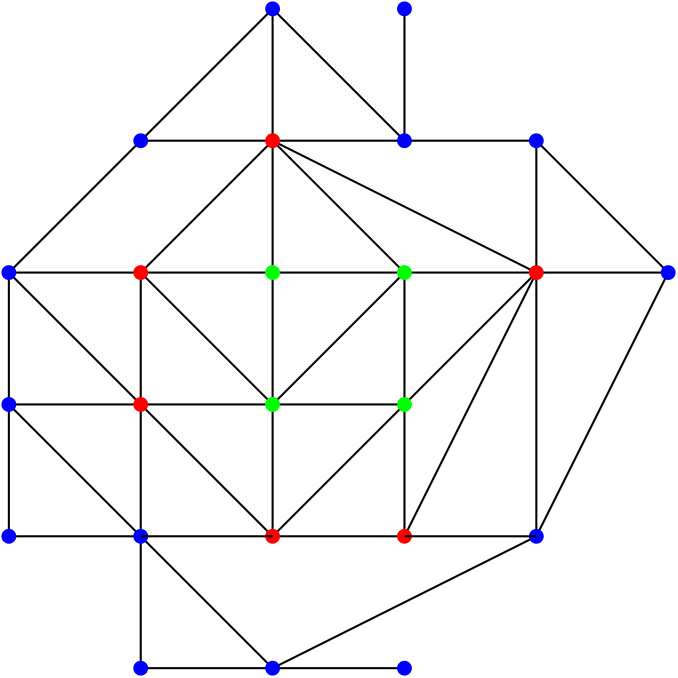
\includegraphics[height=6cm]{images/outer3.png}}
    \end{minipage}
\end{frame}

\begin{frame}{Preparação}
    Dado $G=(V, E)$ planar e $k \in \N^*$, definimos:
    \pause
    \begin{enumerate}[-]
        \item $\ell = k+1$;
        \item Para $0 \le i < \ell$, seja $S_i = \bigcup \{L_j \mid j \equiv i \pmod \ell\}$
        \begin{enumerate}[-]
            \item Ex.: $\ell = 4 \Rightarrow S_1 = L_1 \cup L_5 \cup L_9 \cup \dots$
        \end{enumerate}
        \item $G_i = G[V - S_i]$.
    \end{enumerate}
\end{frame}

\begin{frame}{Decomposição em \emoji{onion}}
    \centering
    \Large $\ell=3$:
    \bigbreak
    \begin{minipage}{\linewidth}
        \centering
        \only<1>{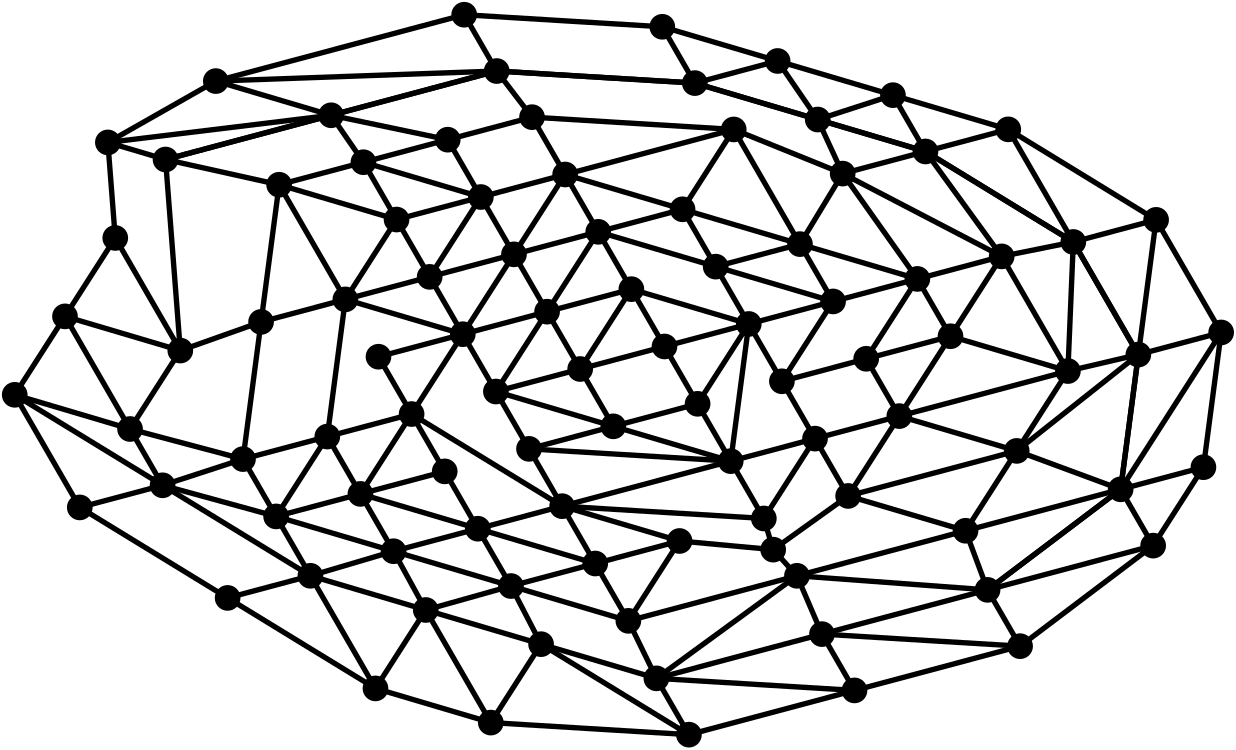
\includegraphics[height=4cm]{images/onion1.png}}
        \only<2>{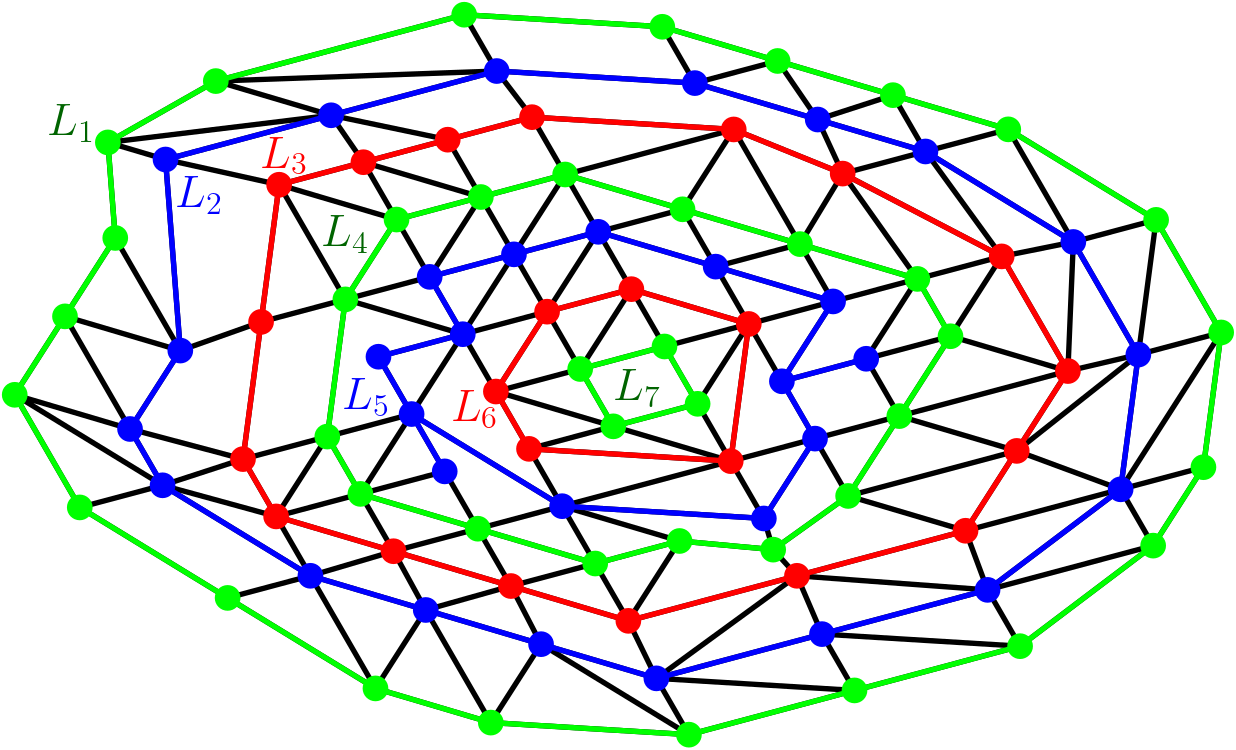
\includegraphics[height=4cm]{images/onion2.png}}
        \only<3>{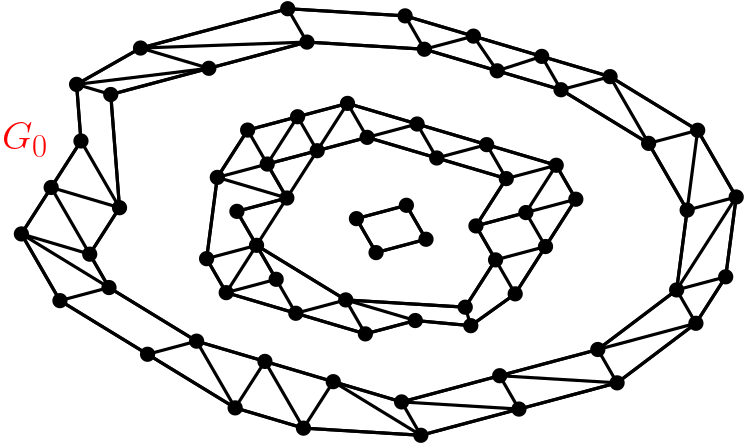
\includegraphics[height=4cm]{images/onion3.png}}
        \only<4>{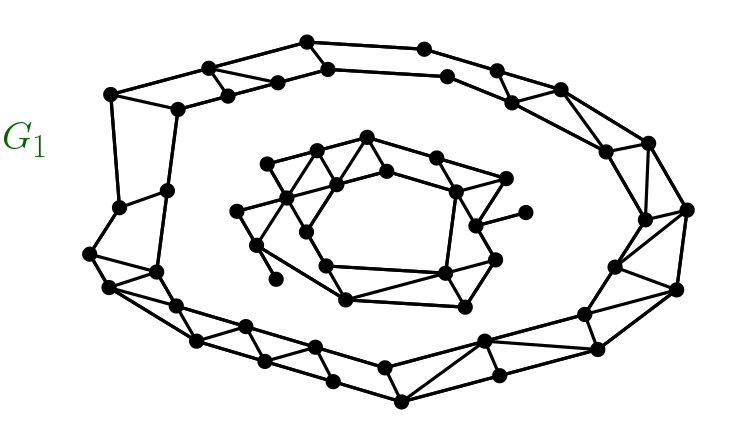
\includegraphics[height=4cm]{images/onion4.png}}
        \only<5>{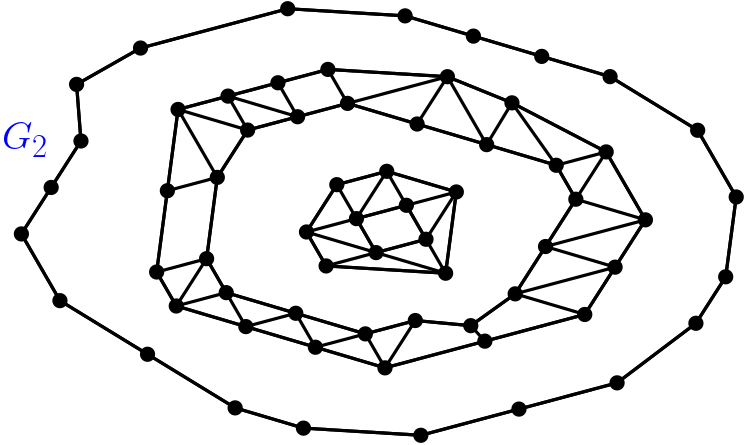
\includegraphics[height=4cm]{images/onion5.png}}
    \end{minipage}
\end{frame}

\begin{frame}{Solucionando $G_i$}
    \centering\Large
    Usamos o Lema 1 em cada componente.
\end{frame}

\begin{frame}{Solução Ótima para $G_i$}
    \centering\Large
    Para cada $i$, geramos uma solução ótima $X_i$ de $G_i$.
    \bigbreak
    O tempo total gasto é $2^{O(k)} \cdot n$.
\end{frame}

\begin{frame}{Solucionando $G$}
    \centering\Large
    Basta retornar o $X_\alpha$ de maior cardinalidade!
\end{frame}

\begin{frame}{Corretude}
    \pause
    \setbeamercovered{transparent} % fade-in/fade-out lists
    \begin{proof}
        \begin{enumerate}
            \setlength\itemsep{1em}
            \item<2,8> Seja $O \subseteq V$ uma solução ótima;
            \item<3,8> Suponha que $|O| \ge k$;
            \item<4,8> $S_0, \dots, S_{\ell-1}$ particionam $V$;
            \item<5,8> Algum $i$ satisfaz $|O \cap V(G_i)| \ge k$;
            \item<6,8> $O \setminus S_i$ é independente em $G_i$;
            \item<7,8> Então $|X_\alpha| \ge |O \setminus S_i| = |O \cap V(G_i)| \ge k$.
        \end{enumerate}
        \alt<8>{\qedhere}{\phantom\qedhere}
    \end{proof}
\end{frame}
